%=====================================================================
\section{Method 1: the MILP (exact model, Gurobi)}

\subsection{What a MILP is}

A MILP writes the problem as equations. Yes/no decisions become 0/1 variables (``car 7 uses gun 3 of station 5'', ``van 2 drives from car 7 to car 12''), times become continuous variables, and every rule becomes a linear inequality (``a gun charges one car at a time'', ``the van's battery covers its route''). The software Gurobi then searches through the possible plans with \emph{branch and bound}: it solves easier versions of the problem to get a lower bound on the cost, and keeps the best plan found so far. When the best plan meets the bound, the plan is \emph{proven optimal}.

Formulation 4 has exactly the variables and the 22 rules of formulation 3 (equations (2)--(23) of \code{formulation\_4.pdf}); only each customer's cost coefficients change with segment and income. It is the \textbf{complete model}: every gun and every van is available to every car; nothing is simplified.

\subsection{How it was run}
\begin{itemize}
  \item 300 seconds per instance, 4 threads, 8 instances at a time on the 32-core server;
  \item the greedy plan (when the greedy rule finds one) is given to Gurobi as a starting point;
  \item every result is one of four: \textbf{optimal}; \textbf{time limit with a plan} (best plan found, with its gap); \textbf{time limit without a plan} (no valid plan found in 300 s); \textbf{infeasible} (proven: no plan can satisfy all rules);
  \item every plan is re-checked by an independent checker (\code{common/check\_plan\_f4.py}), which recomputes $Z$ and all rules.
\end{itemize}

\inshort{The MILP gives the best possible plan when it can prove it, a good plan with a known gap when it runs out of time, and nothing when even a first plan is too hard to find in 300 seconds.}

%=====================================================================
\section{Method 2: reinforcement learning}
\label{sec:rlmethod}

\subsection{The idea}

Instead of solving each instance from scratch, a neural network \emph{learns how to build good plans}. It is trained once, on many random instances made with the same rules as the dataset, and then builds a plan for any new instance in a fraction of a second. The method is the one of RL1 (formulation 3), rebuilt for formulation 4; it is based on the Attention Model (Kool et al.\ 2019), POMO (Kwon et al.\ 2020) and the two-step decoder of Li et al.\ (2021). The full explanation, with all papers and proofs, is in \code{RL2\_reinforcement\_learning\_method\_2/reports/RL\_implementation\_report.pdf}.

\subsection{Building a plan step by step}

The plan is built one decision at a time. Each decision is a pair: \emph{``car $i$ goes next to resource $k$''}, where $k$ is one of the 24 guns or one of the 5 vans. The car is added at the end of that gun's queue or that van's route. A \textbf{simulator} does everything that can be computed:
\begin{itemize}
  \item \textbf{times}: the session starts as early as possible (at the gun: when the car has arrived and the gun is free; with a van: when the van has arrived and the car has requested). Once the order is fixed this is always the best timing, because every time cost grows with a later start;
  \item \textbf{rules (masks)}: a pair is offered only if it breaks no rule: the station is within range, the queue is not longer than $W_i$, the car is charged by $T$; the van has a free seat, enough battery to charge this car and still get home, and is back by $T$;
  \item \textbf{cost}: the exact increase of $Z$ caused by the decision. Over a whole plan these increases add up exactly to $Z$.
\end{itemize}
If a car is left with no allowed option, it is counted as unplaced and the plan is reported as invalid.

\begin{figure}[H]
\centering
\begin{tikzpicture}[font=\footnotesize,
  box/.style={draw=headblue!70,fill=blue!4,rounded corners=2pt,align=center,minimum height=8mm,inner sep=3pt},
  data/.style={draw=black!40,fill=black!3,rounded corners=2pt,align=center,minimum height=7mm,inner sep=3pt},
  arr/.style={-{Stealth[length=2.2mm]},thick,draw=black!60}]
\node[data] (ev) at (-4.2,0) {car features\\ 19 per car};
\node[data] (st) at (0,0) {station features\\ 4 per station};
\node[data] (dep) at (4.2,0) {depot features\\ 4};
\node[box,text width=11.2cm] (enc) at (0,-1.7) {\textbf{Encoder} (reads the whole instance once): every car, station and the depot becomes a vector of 128 numbers; 3 attention layers let every vector take in information from all the others};
\draw[arr] (ev) -- (ev |- enc.north);
\draw[arr] (st) -- (enc);
\draw[arr] (dep) -- (dep |- enc.north);
\node[box,text width=5.3cm] (d1) at (-3.0,-4.0) {\textbf{Step 1: which car next?}\\ looks at all unplaced cars, their cheapest option and how much worse their second-best option is; gives each car a probability};
\node[box,text width=5.3cm] (d2) at (3.0,-4.0) {\textbf{Step 2: which gun or van?}\\ for the chosen car: looks at every allowed gun and van, its free time, battery, seats and the exact cost increase; gives each a probability};
\draw[arr] (enc.south -| d1) -- (d1.north);
\draw[arr] (enc.south -| d2) -- (d2.north);
\draw[arr] (d1.east) -- node[above,font=\scriptsize]{car $i$} (d2.west);
\node[box,text width=11.2cm,fill=orange!6,draw=orange!70] (env) at (0,-6.0) {\textbf{Simulator}: adds car $i$ to gun or van $k$, earliest start time, cost increase, new allowed options};
\draw[arr] (d1) -- (d1 |- env.north);
\draw[arr] (d2) -- (d2 |- env.north);
\draw[arr,dashed] (env.east) -- ++(0.35,0) |- node[pos=0.25,right,font=\scriptsize,align=left]{next\\ car} (d2.east);
\end{tikzpicture}
\caption{The RL policy. The encoder runs once per instance; steps 1 and 2 and the simulator run once for every car placed.}
\label{fig:arch}
\end{figure}

\subsection{The network (architecture)}

\begin{itemize}
  \item \textbf{Inputs.} Each car is described by 19 numbers: its position, request time, charging times at a station and by a van, energy, queue tolerance, income, whether it is stranded, how many stations it can reach and how far the nearest is, how far it is from the depot, its cheapest station option and van option, how late a van may come, and three numbers new in formulation 4: \emph{commercial or not}, its money sensitivity $\mu$, and the cost of queueing for one charging duration ($c^Q\tau^F$). Each station has 4 numbers (position, guns, share of cars that can reach it), the depot 4 (seats per car, guns per car, length of the period, size). All numbers are scaled (by $T$, the battery, the city size or the instance's typical cost) so that small and large, short and long instances look alike to the network.
  \item \textbf{Encoder.} A Transformer of 3 layers, 8 attention heads, vectors of 128 numbers. Attention is a weighted average: each car's vector is updated with a mix of all other vectors, with weights the network learns. There is no fixed order of the cars, so the same network works for 10 or 100 cars.
  \item \textbf{Decoder, step 1 (which car).} Combines the average of the unplaced cars, the depot and 4 numbers about the progress of the plan; scores every unplaced car using its vector plus 7 numbers that change during the construction (options left, cheapest option, regret = second-cheapest minus cheapest, earliest finish, gun versus van cost, how soon it requested, its place in the queue of open requests).
  \item \textbf{Decoder, step 2 (which resource).} For the chosen car, scores every gun (by its station's vector) and every van (by the vector of the place where it now is), plus each resource's state and 6 numbers about the exact pair (its cost increase, its wait, finish, battery left after it).
  \item \textbf{Size.} \frlParams{} learned weights.
\end{itemize}

\subsection{How it learns}
\begin{enumerate}
  \item \textbf{Random training instances} are drawn with the dataset's rules: new positions (clustered, random or mixed), stations by $k$-means, energies, ranges with 15\,\% stranded, request times, and \emph{segment} (70\,\% commercial) and \emph{income} from the calibrated distributions. The 56 test files are never used in training.
  \item \textbf{Warm-up by imitation} (first 500 batches): the network learns to copy the greedy rule (stranded cars first, then by request time, then the cars that hate queueing most; each takes its cheapest allowed option). This gives a sensible start instead of random behaviour.
  \item \textbf{Reinforcement learning} (REINFORCE with a shared baseline): every training instance is solved 8 times by sampling; the plans cheaper than the average of the 8 are made more likely, the dearer ones less likely. 32 instances per batch, 50 batches per epoch.
  \item \textbf{Stopping}: at least 200 epochs; then stop after 10 epochs without a better result on fixed validation instances, at most 500 epochs. The network of the best epoch is kept.
\end{enumerate}

\begin{figure}[H]
\centering
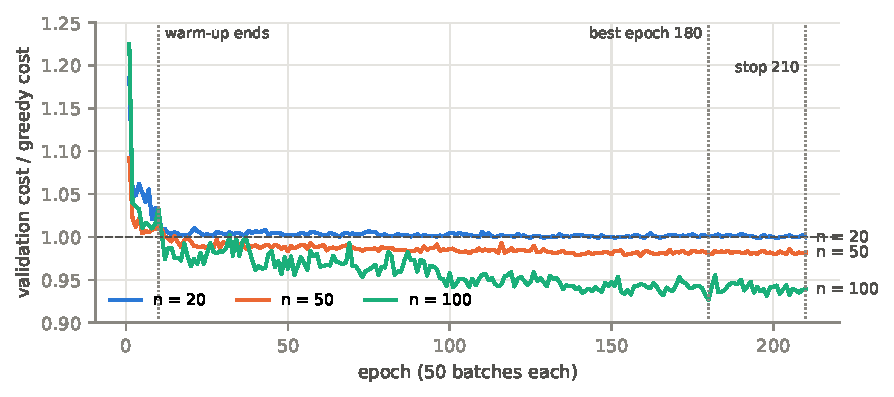
\includegraphics[width=0.88\textwidth]{figures/rl_training.pdf}
\caption{Training of the baseline RL policy: cost of its plans divided by the greedy rule's cost on fixed validation instances (below 1 = better than greedy). Untrained it costs \frlUntrained{} times the greedy rule; after one warm-up epoch \frlAfterWarmOne{}. Best at epoch \frlBestEpoch{} (\frlBestVal); stopped at epoch \frlStopEpoch{} after \frlTrainMin{} minutes on the RTX 4090. The gain over greedy is largest for large instances.}
\label{fig:rltrain}
\end{figure}

\subsection{How it solves a test instance}

The map is turned and mirrored in 8 ways (distances stay the same, but the network sees different coordinates). For each, the policy builds 1 plan taking always its most likely choice and 64 plans by sampling: 520 plans in all. The plan with the fewest unplaced cars, then the lowest $Z$, is kept and scored by the same checker as the MILP.

\subsection{Zero-shot and retrained runs in the experiments}

For each experiment variant RL gives two runs:
\begin{itemize}
  \item \textbf{zero-shot}: the baseline policy, unchanged, applied to the changed data. This works because the network's inputs contain the changed numbers (tariffs and costs through the cost increases, $\mu$, the fleet). It tests whether one trained policy can be reused when an assumption changes;
  \item \textbf{retrained}: a new policy trained from scratch with the variant's values, same recipe (about 39 minutes each, 15 models).
\end{itemize}

\inshort{The RL policy builds a plan car by car, choosing first a car and then a gun or van; a simulator keeps every step legal and exactly costed. It learns once from random examples and then solves any instance in about a tenth of a second.}
